\documentclass[twocolumn]{revtex4}
\usepackage{graphics,graphicx,epsfig,amsmath,multirow,gensymb,commath,textcomp,natbib,blindtext,mhchem,tabularx,array,makecell}
\usepackage[normalem]{ulem}
\newcommand{\squeezeup}{\vspace{-2.5mm}}

\def\bibsection{\section*{\refname}} 
\renewcommand{\thesubsection}{\alph{subsection}}

\renewcommand\theadalign{bc}
\renewcommand\theadfont{\bfseries}
\renewcommand\theadgape{\Gape[4pt]}
\renewcommand\cellgape{\Gape[4pt]}

\begin{document}

\textheight=26.385cm
%Change textheight as the last resort...

\title{Supernova Cosmology: Mid-Term Report}
 
\author{Jacky Cao, AstroLabs, Lab Partner: Duncan Middlemiss \\ Dates of experiment: 19/10/2017 to -, Date of report: 08/11/2017}
\maketitle
\vspace{-3ex}
\subsection*{Project aims} 
\vspace{-2ex}
In studying supernovae and their relation to cosmology we have chosen the following for our project aims:
\begin{itemize}
 \item To observe supernovae using telescopes based in Durham and La Palma over an extended period.
 \item To use collected data and then to perform photometry on that data to produce plots of the magnitude shown as a function of time (with uncertainties as well).
 \item To then apply templates/models to our data and evaluate the quality of our data by performing more analysis eg. $\chi^2$ tests.
 \item Then using our data for Type Ia supernovae, we hope to produce a value for $H_0$. With this value we can again attempt to evaluate the quality of our data.
 \item As part of our extension projects we are hoping to:
 \begin{itemize}
  \item Perform a \em{galaxy subtraction }\em so that we are just left with the SN object, and then try and perform photometry again. Noting the differences in values we achieve for our magnitudes.
  \item Attempting to discover a SN by observing galactic clusters - areas which have potentially have a higher chance for SNe to occur in.
 \end{itemize}
\end{itemize}

\vspace{-3ex}
\subsection*{Progress so far} 
\vspace{-2ex}

Our project has been centred around supernovae, for our experiment we have been attempting to collect enough magnitude data over the past few weeks to generate some light curves. We have been aiming to try and see the characteristic shapes that are associated with the varying types of SN - from Type Ia to Type II. 

To perform our data collection we have been using the telescopes in Durham (on the Physics Department's Roof) and we have used the robotic telescope in La Palma. When there has been an opportunity for us to observe in Durham we have always aimed to use Far-East-16. This is because our objects have been quite faint (having a magnitude of around $\sim 15 - 18$), therefore we require a telescope which can collect as much as light as possible (the 16-inch). But, we can also use East-14 or West-14, we just need to ensure that we use a longer exposure time so that we ensure we are collecting as much light as possible. 

Once we had collected this data, we then perform photometry analysis. After we have copied the data from the data from the remote server, we generally make sure all the frames that we are using are good quality - we can view our objects, and if the image has a lot of noise or not. Once we have decided on which images which we will be using in each band, we perform a stacking routine on them. With the provided d$\_$stack script, we have been combining the images to produce one frame which has a better signal-to-noise ratio. 

In calculating the magnitudes of our objects we have so far been using differential (instrumental) photometry. Our supernova magnitude is calibrated using a zero point which has been found from two calibration stars in the same frame. The equation which is used is 
\begin{equation}
 m = z - 2.5 \log_{10}{C},
 \label{eqn1}
\end{equation}
where $m$ the magnitude of the object, $z$ is the zero-point, and $C$ is the number of counts of the object. 

The uncertainties on this calculated magnitude is found by using,
\begin{equation}
 \delta{m} = 2.5 \log_{10}{\Big(1+\frac{1}{\sqrt{C}}\Big)},
 \label{eqn2}
\end{equation}
where $\delta{m}$ is the uncertainty in the magnitude, and $C$ is the number of counts of our object.

The object we have been focussing this photometry on is 2017hhz. We have five days of data points with uncertainties, and as this is a Type Ia supernova explosion we have managed to fit templates to this using SNooPy. From Figure \ref{2017hhz-snpy} we can see that whilst our data appears to fit the light curve, we cannot be sure if that is the correct location to fit the maximum magnitude at. We require more data to be plotted as well.

\begin{figure}[!h]
\begin{center}
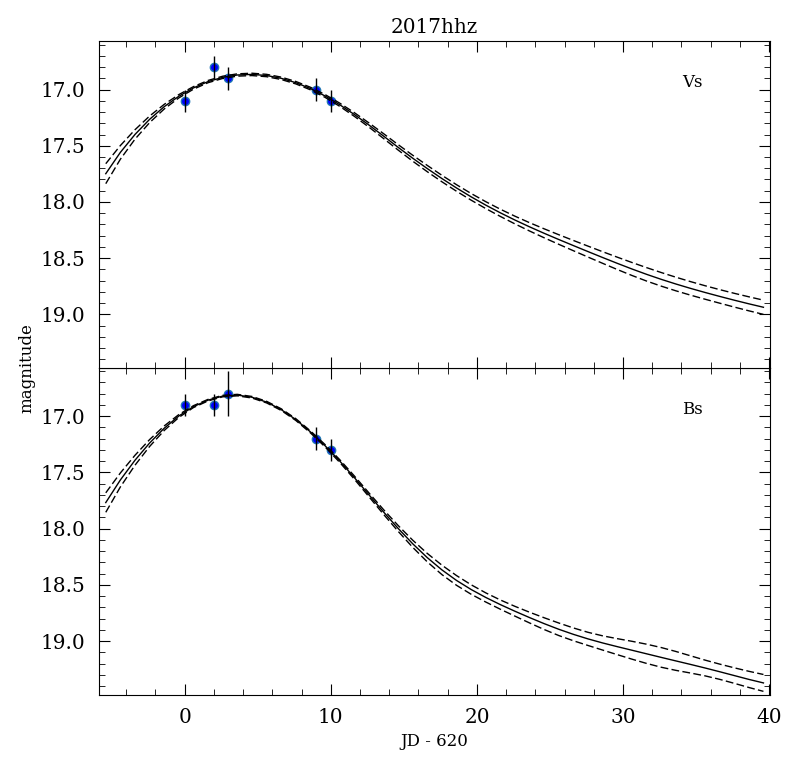
\includegraphics[width=9cm]{figs/2017hhz}
\caption[]{Plot which has been produced by SNooPy - a template for Type Ia supernovae has been fitted to our SNe data for our object 2017hhz in V and B bands. The horizontal axis is the time, the first data point was chosen to be 0 as that was our first data point.}
\label{2017hhz-snpy}
\end{center}
\end{figure}

In Table \ref{2017hhz-table} we can see the data which was used.

\begin{table}[h!]
\centering
\begin{tabular}{c@{\hskip 20pt}c@{\hskip 20pt}c@{\hskip 20pt}c@{\hskip 20pt}c} 
 \hline
 \textbf{Date Observed} & \textbf{$\boldsymbol{m_B}$} & \textbf{$\boldsymbol{\Delta{m_B}}$} & \textbf{$\boldsymbol{m_V}$} & \textbf{$\boldsymbol{\Delta{m_V}}$} \\ [0.5ex] 
 17/10/20 & 16.9 & 0.1 & 17.1 & 0.1 \\
 17/10/22 & 16.9 & 0.1 & 16.8 & 0.1 \\
 17/10/23 & 16.8 & 0.2 & 16.9 & 0.1 \\
 17/10/29 & 17.2 & 0.1 & 17.0 & 0.1 \\
 17/10/30 & 17.3 & 0.1 & 17.1 & 0.1 \\
 \hline
\end{tabular}
\caption{The B and V band magnitudes and their uncertainties for SNe 2017hhz on the given dates. The former values were calculated using equation \ref{eqn1} and the latter using equation \ref{eqn2}.}
\label{2017hhz-table}
\end{table}

\vspace{-3ex}
\subsection*{Plan for the remainder of the project}
\vspace{-2ex}
As we move onto the final weeks of our project, the main question that we would like to ask is: to what accuracy can we produce these light curves to and whether or not it would produce a valid value for Hubble's Constant, $H_0$?

We certainly want to continue observing 2017hhz to see if we can produce a greater fitting of the SNooPy templates to our data. But it would also be interesting to see if we can find observe a SN object which is not a Type Ia, say, a Type II for example, and manually fit a template. 

We will continue to look at the SN databases (Rochester and ASAS-SN) so that we can have more targets to view so to potentially produce light curves which are more well defined. We are currently nearing the limits of the telescopes in terms of how faint an object which can be viewed. Having a $\sim 14$ object would be exciting to work with.

We will also try and find the zero-points for our images using different methods, e.g. using the find$\_$point Python script. With this we want to see how different would our magnitude values be and whether this would produce a better fit for the templates.

It would also be of benefit if we flat-field our images so that we can improve our signal-to-noise ratio further, thus potentially producing data which fits well to the templates.

There is still a lot of work to complete and analysis to perform, but with good time management and planning we will be able to complete our project to some degree.

\bibliographystyle{abbrv}
\bibliography{supernovae}

\clearpage
\onecolumngrid
\vspace{-3ex}
\section*{Appendix A - Objects Log}
\vspace{-2ex}
A list of the objects that were chosen to be observed, and then the subsequent notes on them. Not all objects were chosen to be observed for an extended period, the ones noted were observed for a couple of nights to ensure suitability. The subsequent observation logs can be found in Appendix B.

{\renewcommand{\arraystretch}{1.2}%
\begin{table}[h!]
\centering    
\begin{tabularx}{\textwidth}{c c c c @{\hskip 5pt} c c X}
    \hline
    \textbf{Object} & \textbf{RA} & \textbf{Dec} & \textbf{Magnitude} &\textbf{First Discovered} &\textbf{Type} & \textbf{Notes} \\ 
    *ASASSN-17mz & 23:56:21.82 & 32:27:24.08 & 14.6 & 2017/09/30.500 & Ia & {Too close to galactic nucleus, cannot see}  \\
    *AT2017hld & 22:18:22.849 & 34:45:08.46 & 16.1 & 2017/10/17.339 & CV & {Cataclysmic Variable, stopped observing}  \\
    *AT2017hky & 11:23:30.514 & 63:21:59.43 & 16.2 & 2017/10/16.640 & II & {Not viewable from Durham or La Palma}  \\
    2017hhz & 01:44:16.75 & 12:15:18.00 & 16.83 & 2017/10/16.140 & Ia & {A measured redshift, $z=0.0392$}  \\
    AT2017gvb & 08:04:42.34 & 61:31:41.50 & 17.33 & 2017/09/26.59 & unk & {-}  \\
    *ASASSN-17nb & 07:27:37.32 & 35:36:28.30 & 17.31 & 2017/09/25.59 & II & {Object is dwarfed by brightness of the galaxy}  \\
    2017hle & 01:07:36.060 & 32:24:30 & 18.0 & 2017/10/18.684 & Ia-91bg & {-}  \\
    2017hou & 04:09:02.140 & -01:09:36.40 & 17.9 & 2017/10/24.370 &Ia & {Viewable from La Palma}  \\
    *AT2017hmw & 01:07:16.570 & 31:25:28.88 & 17.2 & 2017/10/19.415 & CV & {Cataclysmic Variable}  \\
    2017hpa & 04:39:50.750 & 07:03:54.90 & 17.9 & 2017/10/15.346 & Ia & {Viewable from La Palma}  \\
    *AT2017hnm & 01:42:03.24 & 42:31:08.50 & 16.69 & 2017/10/23.44 & unk & {Another star in the image dwarfs the SN in brightness}  \\
    AT2017hpm & 08:04:15.100 & -00:03:58.03 & 16.4 & 2017/10/26.290 & unk & {-}  \\
    *AT2017hqa & 01:08:59.160 & 32:38:04.10 & 17.3 & 2017/10/26.740 & unk & {Unobservable, too close to galactic centre}  \\
    2017hqc & 23:23:08.210 & 10:38:54.63 & 18.0 & 2017/10/27.490 & Ia & {-}  \\
    *AT2017hrr & 11:29:06.490 & -08:59:18.56 & 15.4 & 2017/10/30.607 & unk & {Cannot view from Durham or La Palma}  \\
    *AT2017hhq & 00:42:50.230 & 41:15:27.10 & 17.7 & 2017/10/30.599 & NV & {A nova close to M31}  \\
    AT2017htb & 22:09:38.520 & 17:39:39.56 & 15.7 & 2017/11/02.190 & unk & {-}  \\
    \hline      
\end{tabularx}
\caption{Objects that we chose to observe and notes on them. RA is the Right Ascension, given in units of hours : arcminutes : arcseconds. Dec is the Declination, degrees : minutes : seconds. The stated magnitude is the initial magnitude that the object was discovered in the V band. Objects marked with an asterisk $*$ were objects which we chose to stop observing, the reason provided in the notes.}
\label{objects}
\end{table}


\clearpage

\onecolumngrid
\vspace{-3ex}
\section*{Appendix B - Observation Logs} \label{obslogs}
\vspace{-2ex}
Given below are all the observations which were made during our observation periods. The exposures column is of the following format: ($x: y, z$ s), where $x$ is the band in which the images were taken in, $y$ the number of exposures taken, and $z$ the exposure time which was used, in units of seconds.
{\renewcommand{\arraystretch}{1.2}%
\begin{table}[h!]
\centering    
\begin{tabularx}{\textwidth}{c@{\hskip 5pt} c c@{\hskip 5pt} c@{\hskip 5pt} c@{\hskip 5pt} X}
    \hline
    \textbf{Date} & \textbf{Object} & \textbf{Time} & \textbf{Exposures} & \textbf{  Conditions  } & \textbf{Notes} \\ 
    20/10/17 & 2017hhz & 22:25:34 to 22:58:50 & \makecell{B: 5, 120s \\ V: 5, 120s} & {Clear} & {pt5m: -}  \\
    	& ASASSN-17nb &  02:56:08 to 03:23:36 & \makecell{B: 5, 60s \\ V: 5, 60s} & {Cloudy} & {pt5m: Images produced have a lot of noise.} \\      
	
    21/10/17 & - & - & - & Cloudy & {\em No observations: weather not sufficient in Durham or La Palma for observations. \em} \\
    
    22/10/17 & AT2017hmw &  21:52:20 to 22:31:49 & \makecell{B: 5, 120s \\ V,: 5, 120s} & {Clear} & {pt5m: -} \\  
    & 2017hhz & 22:40:20 to 23:19:50 & \makecell{B: 4, 60s \\ V: 12, 60s} & {Clear} & {pt5m: -}  \\
    & ASASSN-17nb &  02:42:45 to 03:10:46 & \makecell{B: 5, 120s \\ V: 5, 60s} & {Clear} & {pt5m: -} \\  
    & AT2017gvb & 03:12:31 to 03:58:58 & \makecell{B: 5, 180s \\ V: 5, 120s} & {Clear} & {pt5m: -} \\    
    
    23/10/17 & 2017hhz & 22:53:12 to 23:32:42 & \makecell{B: 5, 120s \\ V: 5, 120s} & {Cloudy} & {pt5m: Data produced has FWHM ranging from $1.6$ to $9.9$.} \\  
    
    24/10/17 & 2017hhz & 22:44:01 to 23:23:30 & \makecell{B: 5, 120s \\ V: 5, 120s} & {Cloudy} & {pt5m: Data is noisy, potentially another object transited across the frame while observing.} \\  
    
    25/10/17 & - & - & - & {Cloudy} & {\em No observations: too cloudy for observations in Durham, and items in pt5m queue were pushed out in favour of other objects. \em} \\
    
    26/10/17 & 2017hle & 20:54:44 to 21:09:03 & \makecell{B: 4, 60s \\ V: 4, 60s} & {Clear} & {FE16: - }  \\
    & 2017hhz &  21:18:00 to 21:25:31 & \makecell{B: 4, 60s \\ V: 4, 60s} & {Clear} & {FE16: -} \\ 
    & AT2017hmw &  21:29:15 to 21:39:36 & \makecell{B: 4, 60s \\ V: 4, 60s} & {Cloudy} & {FE16: -} \\
    & Messier-7 &  21:50:23 to 21:54:47 & {C: 1, 60s} & {Slightly Cloudy} & {FE16: Test object for SN discovery.} \\
    & Messier-10 &  21:55:47 to 22:00:13 & {C: 1, 60s} & {Cloudy} & {FE16: Test object for SN discovery.} \\
    & AT2017hnm &  23:27:22 to 23:41:55 & \makecell{B: 5, 120s \\ V: 3, 120s} & {Clear} & {pt5m: -} \\ 
    & AT2017gvb &  - & - & {-} & {pt5m: Object pushed out of the queue in favour of others.} \\

    27/10/17 & AT2017hqa & 18:48:12 to 18:52:59 & \makecell{B: 4, 60s} & {Cloudy} & {FE16: Object too close to galactic nucleus. }  \\
    & AT2017hnm &  18:56:34 to 19:00:23 & \makecell{C: 1, 60s} & {Slightly Cloudy} & {FE16: Object too dim, cloud cover reduced light we were receiving.} \\
    & Abell 426 &  19:04:23 to 19:15:41 & \makecell{C: 1, 60s \\ B: 9, 60s \\ V: 9, 60s} & {Clear} & {E14: Object to observe to discover new SN.} \\
    & 2017hhz &  20:11:35 to 20:22:43 & \makecell{B: 4, 60s \\ V: 4, 60s} & {Cloudy and Windy} & {E14: Seeing is bad due to the weather.} \\
    & 2017hle &  20:26:18 to 20:37:35 & \makecell{B: 4, 90s \\ V: 4, 90s} & {Slightly Cloudy} & {E14: Seeing is bad in these images as well.} \\
    & 2017hou &  23:48:09 to 23:50:14 & \makecell{B: 2, 120s} & {-} & {pt5m: Only two frames taken, not sufficient data.} \\
    \hline      
\end{tabularx}
\label{obs_logs1}
\end{table}

{\renewcommand{\arraystretch}{1.2}%
\begin{table}[h!]
\centering    
\begin{tabularx}{\textwidth}{c@{\hskip 5pt} c c@{\hskip 5pt} c@{\hskip 5pt} c@{\hskip 5pt} X}
    \hline
    \textbf{Date} & \textbf{Object} & \textbf{Time} & \textbf{Exposures} & \textbf{  Conditions  } & \textbf{Notes} \\ 
    27/10/17 & AT2017gvb &  02:16:01 to 03:03:05 & \makecell{B: 5, 120s \\ V: 5, 120s} & {Clear/Cloudy} & {pt5m: Some images are more noisy due to clouds.} \\
    
    28/10/17 & AT2017hnm &  21:41:55 to 22:21:25 & \makecell{B: 5, 120s \\ V: 5, 120s} & {Clear} & {pt5m: -} \\
    & 2017hhz &  21:28:50 to 21:30:50 & \makecell{B: 1, 120s} & {Clear} & {pt5m: -} \\
    
    29/10/17 & 2017hle &  21:22:39 to 21:41:21 & \makecell{B: 10, 120s \\ V: 1, 120s} & {Clear} & {pt5m: Mistake on our part to take so many images in B band, and only one in V band.} \\
    & AT2017hnm &  21:55:34 to 22:35:04 & \makecell{B: 5, 120s \\ V: 5, 120s} & {Slightly Cloudy} & {pt5m: -} \\
    & 2017hhz &  23:16:48 to 23:56:18 & \makecell{B: 5, 120s \\ V: 5, 120s} & {Clear} & {pt5m: -} \\
    & 2017hou &  00:33:33 to 01:13:02 & \makecell{B: 5, 120s \\ V: 5, 120s} & {Clear} & {pt5m: -} \\
    & 2017hqc &  01:16:20 to 01:41:20 & \makecell{B: 4, 120s \\ V: 4, 120s} & {Clear} & {pt5m: -} \\
    & AT2017gvb &  02:18:51 to 02:55:47 & \makecell{V: 13, 180s} & {Clear} & {pt5m: Long exposure and large number of exposures chosen as a test to see the quality of stacking them.} \\
    
    30/10/17 & 2017hle &  21:18:56 to 21:58:25 & \makecell{B: 10, 120s \\ V: 10, 120s} & {Clear} & {pt5m: -} \\
    & 2017hhz &  22:06:34 to 22:46:04 & \makecell{B: 5, 120s \\ V: 5, 120s} & {Clear} & {pt5m: -} \\
    & AT2017gvb &  02:04:22 to 03:02:50 & \makecell{V: 20, 180s} & {Clear} & {pt5m: An human error, we re-selected this object from the previous night instead of the one with the correct number of required frames for each band.} \\
    
    31/10/17 & - & - & - & {Cloudy} & {\em No observations: too cloudy for observations in Durham and La Palma. \em} \\
    
    01/11/17 & 2017hle & 23:56:53 to 00:15:35 & \makecell{B: 5, 120s \\ V: 5, 120s} & Clear & {pt5m: -} \\
    & AT2017hnm & 00:18:23 to 00:57:55 & \makecell{B: 5, 120s \\ V: 5, 120s} & Clear & {pt5m: -} \\
    & 2017hhz & 01:00:47 to 01:40:17 & \makecell{B: 5, 120s \\ V: 5, 120s} & Clear & {pt5m: -} \\
    & 2017hou & 01:43:38 to 02:23:08 & \makecell{B: 5, 120s \\ V: 5, 120s} & Clear & {pt5m: -} \\
    
    02/11/17 & - & - & - & {Cloudy} & {\em No observations: too cloudy for observations in Durham and La Palma. \em} \\
    
    03/11/17 & - & - & - & {Cloudy} & {\em No observations: too cloudy for observations in Durham and La Palma. \em} \\
    
    04/11/17 & - & - & - & {Cloudy} & {\em No observations: too cloudy for observations in Durham and La Palma. \em} \\
    
   05/11/17 & ASASSN-17mz & 17:53:45 to 18:09:34 & \makecell{B: 8, 60s \\ V: 8, 60s} & {Clear} & {FE16: -} \\
   & 2017hhz & 18:50:39 to 19:24:43 & \makecell{B: 8, 120s \\ V: 8, 60s} & {Clear} & {FE16: -} \\
   & AT2017htb & 19:38:14 to 20:02:16 & \makecell{B: 8, 60s \\ V: 8, 60s} & {Slightly Cloudy} & {W14: -} \\
   & 2017hle & 20:05:49 to 20:08:28 & \makecell{V: 2, 60s} & {Cloudy} & {W14: Stopped taking exposures after viewing the weather.} \\
   & 2017hqc & 20:14:16 to 20:18:25 & \makecell{V: 3, 60s} & {Cloudy} & {W14: Seeing if images will be strongly affected by the cloud cover.} \\
   & AT2017hhq & 20:33:58 to 20:42:26 & \makecell{B: 4, 60s \\ V: 4, 60s} & {Clear} & {W14: -} \\
       \hline      
\end{tabularx}
\label{obs_logs2}
\end{table}

{\renewcommand{\arraystretch}{1.2}%
\begin{table}[h!]
\centering    
\begin{tabularx}{\textwidth}{c@{\hskip 5pt} c c@{\hskip 5pt} c@{\hskip 5pt} c@{\hskip 5pt} X}
    \hline
    \textbf{Date} & \textbf{Object} & \textbf{Time} & \textbf{Exposures} & \textbf{  Conditions  } & \textbf{Notes} \\ 
    05/11/17 & AT2017hhq & 19:38:14 to 20:02:16 & \makecell{B: 3, 30s \\ V: 3, 30s \\ R: 3, 30s} & {Cloudy} & {E14: Images taken so that we can produce a colour image. } \\
    
    06/11/17 & - & - & - & {Cloudy, and Rain} & {\em No observations: too cloudy for observations in Durham, and torrential rain in La Palma. \em} \\
    
    07/11/17 & - & - & - & {Cloudy and Rain} & {\em No observations: too cloudy for observations in Durham, and torrential rain in La Palma. \em} \\
    
    08/11/17 & - & - & - & {Cloudy and Rain} & {\em No observations: too cloudy for observations in Durham, and torrential rain in La Palma. \em} \\
    
       \hline      
\end{tabularx}
\caption{Observing logs for the our experiment up to the 8th November 2017.}
\label{obs_logs3}
\end{table}


\clearpage

\end{document}